%!TEX root = ../../main.tex
\section{Modellentwicklung}
Die Entwicklung des \gls{Modell}s ist ein anspruchsvolles Unterfangen, das im folgenden Kapitel näher erläutert wird. Zunächst wird die Architektur des \gls{Modell}s vorgestellt und wie es aufgebaut ist. Im nächsten Punkt wird erklärt, was Hyperparameter sind und was sie bewirken, gefolgt von den Problemen bei der Entwicklung und der Implementierung mit PyTorch. Abschließend wird der Trainingsprozess beschrieben.
\subsection{Architektur des Neuronalen Netzes}
\label{sec:Modellarchitektur}
Die gewählte Architektur ist ein U-Net, das seinen Namen seiner U-förmigen Struktur verdankt (siehe Abb. \ref{fig:unet_aufbau}). Das U-Net wurde speziell für die Segmentierung biomedizinischer Bilder entwickelt und ist eine Sonderform des \ac{CNN}s. Das U-Net ist speziell darauf ausgelegt, auch mit kleinen Datensätzen gute Ergebnisse zu erzielen. In der Medizin stehen oft nur begrenzt beschriftete Daten zur Verfügung, da der Aufwand für die Beschriftung der Daten hoch ist. Aufgrund dieser Tatsache ist U-Net für diese Zwecke besonders geeignet. Die folgende Beschreibung der Architektur basiert auf dem originalen U-Net und wird in dieser Arbeit als Basis für das \gls{Modell} verwendet, welches im Abschnitt \ref{subsec:Implementierung} genauer beschrieben wird.

\begin{figure}
	\centering
	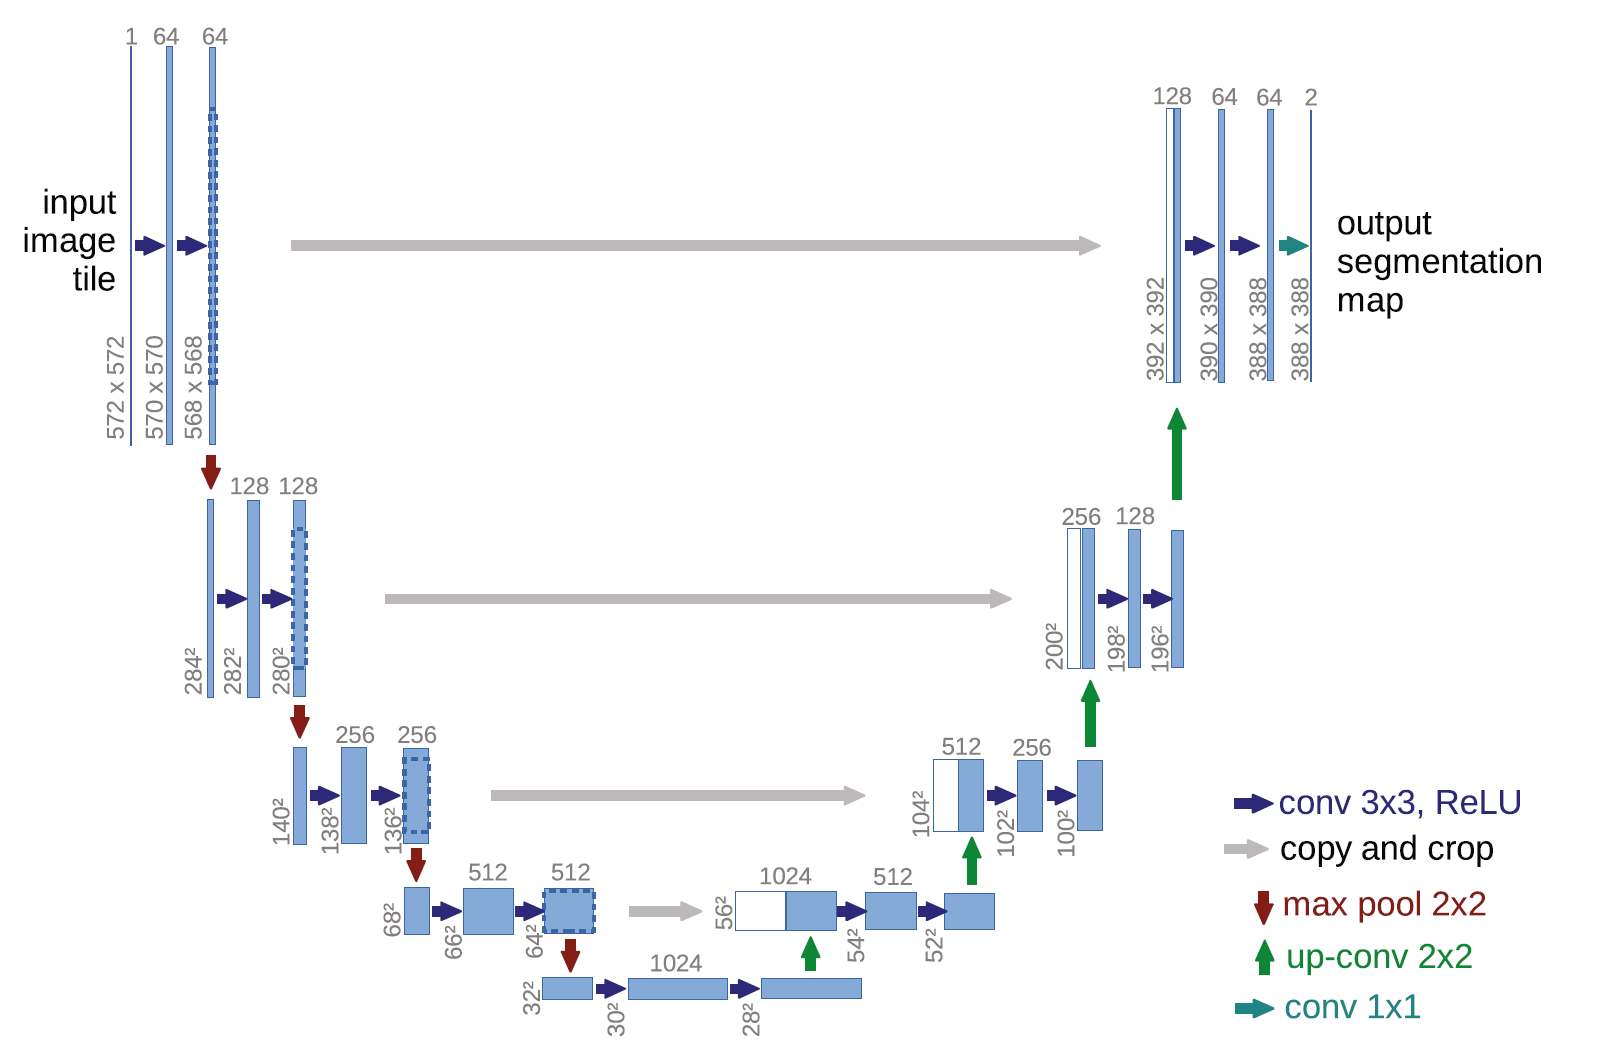
\includegraphics[width=.9\textwidth]{unet_aufbau.png}
	\caption{Aufbau eines U-Nets mit einem Encoder und Decoder Abschnitt für die Extrahierung von Merkmalen und die Wiederherstellung des Original Bildes mit der fertigen Segmentierung (Quelle: \cite{Ronneberger2015})}
	\label{fig:unet_aufbau}
\end{figure}
Die Architektur des Netzes besteht aus zwei Teilen, dem Downsampling-Pfad, auch Encoder genannt, und dem Upsampling-Pfad, auch Decoder genannt. Der Encoder ähnelt einem klassischen \ac{CNN} und besteht aus einer Reihe von Convolutional- und Max-Pooling-Operationen, aber es gibt keine vollständig vernetzten Schichten. 

Der Encoder wird verwendet, um die Feature-Maps aus dem Bild zu extrahieren. Mit jedem Eingabeschritt des Encoders werden mehr Feature-Maps extrahiert und die räumliche Dimension des Bildes reduziert. Die Ausgabe wird an die nächsthöhere Schicht weitergeleitet, um so viele Details wie möglich auf verschiedenen Ebenen zu erhalten. Die Struktur besteht aus einer Reihe von Doppelfaltungen mit einem 3x3-Filter, gefolgt von einer Max-Pooling-Schicht mit einer Filtergröße von 2x2 und einer Schrittweite von 2. In jedem Encoderschritt wird die Anzahl der Filter bzw. Feature-Maps in den Faltungsschichten verdoppelt.

Im Decoder wird die komprimierte Eingabe wieder auf die ursprüngliche Bildgröße skaliert, auch ''Upsampling`` genannt. Dies geschieht durch eine Abfolge von Upsampling-Layern, jeweils gefolgt von einer zweimaligen Faltung und einer Aktivierungsfunktion. Nach jedem Upsampling der Feature-Maps folgt eine Faltung mit einem $2\times2$-Filter, wodurch die Anzahl der Feature-Maps jeweils halbiert wird. Hierbei findet zusätzlich eine Verkettung der Feature-Maps aus dem entsprechenden Encoderabschnitt statt. Nach der $2\times2$ Faltung folgen immer zwei $3\times3$ Faltungen mit einer abschließenden ReLU Aktivierungsfunktion. Nach dem Decoder-Abschnitt folgt noch eine Faltung mit einem $1\times1$-Filter, der die Merkmale auf die gewünschte Anzahl von Klassen der Segmentierungsaufgabe abbildet. \cite[vgl.][]{Ronneberger2015}

\subsection{Hyperparameter}
Hyperparameter sind Parameter, deren Werte vor dem Training eines \gls{Modell}s festgelegt werden und die, von Ausnahmen abgesehen, während des Trainings nicht angepasst werden. Sie sind entscheidend für die Leistungsfähigkeit des Modells und müssen sorgfältig ausgewählt werden. Die Wahl der richtigen Hyperparameter ist oft eine Kunst, die Erfahrung und experimentelles Ausprobieren erfordert. 

In der Praxis wird häufig eine Technik namens Hyperparametersuche oder -optimierung verwendet, bei der verschiedene Kombinationen von Hyperparametern systematisch ausprobiert werden, um diejenige zu finden, die die beste Leistung liefert. In diesem Abschnitt werden die wichtigsten Hyperparameter, die bei der Entwicklung eines Deep Learning \gls{Modell}s relevant sind, näher beschrieben.

\paragraph{Lernrate} Die Lernrate ist ein entscheidender Hyperparameter in fast allen Optimierungsalgorithmen für neuronale Netze. Sie bestimmt, wie stark die Gewichte des Netzes in jedem Trainingsschritt angepasst werden. Eine zu hohe Lernrate kann dazu führen, dass das globale Minimum der Verlustfunktion übersprungen wird und das \gls{Modell} möglicherweise nicht konvergiert. Bei einer zu niedrigen Lernrate wird der Fehler nur um sehr kleine Werte reduziert, was zu einer langsamen Konvergenz führt. Es kann auch vorkommen, dass der Fehler um einen Wert oszilliert und somit bei einer suboptimalen Lösung hängen bleibt. \cite[vgl.][]{Pfannstiel2022}

\paragraph{Batch Größe} Die Batch-Größe bezieht sich auf die Anzahl der Trainingsbeispiele, die das Netz gleichzeitig sieht, bevor es seine Gewichte aktualisiert. Eine größere Batch-Größe kann zu einer stabileren Aktualisierung der Gewichte führen, benötigt jedoch mehr Speicherplatz und verlangsamt das Training. Eine kleinere Batchgröße kann zu einem schnelleren, aber weniger stabilen Training führen. Übliche Batchgrößen reichen von 2, 8, 16 bis hin zu Hunderten von Bildern in einem Batch. \cite[vgl.][]{Yu2020}

\paragraph{Anzahl der Epochen} Eine Epoche bezeichnet einen Durchlauf des gesamten Datensatzes während des Trainings. Die Anzahl der Epochen, für die das \gls{Modell} trainiert wird, beeinflusst die Fähigkeit des Modells, Muster aus den Daten zu lernen. Es ist wichtig, eine geeignete Anzahl von Epochen auszuwählen, um einen optimalen Trainingsprozess zu erhalten. Ist die Anzahl der Epochen zu gering, hat das Netz nicht genügend Zeit, um wichtige Muster zu lernen, was zu Underfitting führen kann. Ist die Anzahl der Epochen hingegen zu hoch, besteht die Gefahr, dass sich das Netz zu stark an die Trainingsdaten anpasst und es zu einem Overfitting kommt. \cite[vgl.][]{Goodfellow2016}

\paragraph{Architektur spezifische Parameter} Im Kontext der U-Net Architektur gibt es auch spezifische Hyperparameter, die bei der Entwicklung des \glspl{Modell}s berücksichtigt werden müssen, wie z.B. die Anzahl und Größe der Filter in den Faltungsschichten, die Tiefe des Netzes und die Art der Aktivierungsfunktionen.


\subsection{Implementierung}
\label{subsec:Implementierung}
Die Implementierung des \gls{Modell}s zur Segmentierung von Hirntumoren erfolgt in Python mit PyTorch und basiert auf der in \ref{sec:Modellarchitektur} beschriebenen U-Net-Architektur. Die Implementierung weicht in kleinen Teilen von der ursprünglichen U-Net Architektur ab. Die grobe Struktur des U-Net mit jeweils vier Down- und Upsampling-Layern wurde weitestgehend übernommen.

\subsubsection{Padding}
Durch die Faltungen innerhalb des neuronalen Netzes wird die Bildgröße reduziert, da keine Fülldaten verwendet werden. Um dem entgegenzuwirken, wird für eine bessere Implementierung an jedem Bildrand eine bestimmte Anzahl von Pixeln hinzugefügt. Da die Bildgröße aufgrund der gegebenen Architektur bekannt ist (siehe Abschnitt \ref{paragraph:GrößenSkalierung}), kann die Formel \ref{eq:conv_size} zur Berechnung der Füllmenge $P$ verwendet werden. Die Bildgröße $W$ wird durch ein Vielfaches von $2^N$ definiert, wobei $N$ die Anzahl der Downsampling-Schichten beschreibt. In diesem Fall ist $N=4$ und die Eingabegröße der Bilder ist 128x128 Pixel, was ein Vielfaches von $2^N=2^4=16$ ist. Die Schrittweite $S$ und die Filtergröße $F$ sind durch die Konstruktion des U-Netzes mit $S=1$ und $F=3$ bereits vorgegeben. Daraus ergibt sich die Füllmenge mit der Formel \ref{eq:conv_size}:
\begin{equation}
	P = \dfrac{W \cdot S - 1 - W + F}{2}
\end{equation}

\begin{equation}
	P = \dfrac{2^N \cdot 1 - 1 - 2^N + 3}{2}  = 1
\end{equation}
Da die Eingabegröße erhalten bleibt, ist die Implementierung aufgrund der einfachen Berechnung der Bildgröße für jede Schicht vorteilhaft.

\subsubsection{Batch Normalisierung}
Die Batch-Normalisierung ist eine Technik, die häufig im Deep Learning verwendet wird, um das Training zu beschleunigen und die Stabilität des Netzes zu erhöhen. Bei der Batch-Normalisierung werden die Eingaben für jede Schicht normalisiert, indem die durchschnittliche Aktivierung auf 0 und die Standardabweichung der Aktivierung auf 1 gesetzt wird.\\
Normalerweise wird der Mittelwert und die Standardabweichung für jede Batch berechnet, daher der Name Batch-Normalisierung. Es hat sich gezeigt, dass durch die Batch-Normalisierung höhere Lernraten verwendet werden können und das Training im Allgemeinen schneller und effektiver ist. Außerdem wird die Stabilität des Netzes erhöht und die Notwendigkeit einer sorgfältigen Initialisierung der Modellparameter entfällt. Die Schicht fungiert auch teilweise als eine Art Dropout, bei dem das Modell bestimmte Neuronen ``vergisst'' und neu initialisiert, um Overfitting zu vermeiden.\cite[vgl.][]{Ioffe2015}
PyTorch stellt bereits eine Batch-Normalisierungsschicht zur Verfügung, die für die Batch-Normalisierung verwendet werden kann. Diese Schicht wird nach jeder Faltung und vor der Aktivierungsfunktion angewendet.

\subsection{Verlustfunktion}
Die Wahl der richtigen Verlustfunktion ist entscheidend für den Erfolg eines Neuronalen Netzes. Bei der Klassifikation medizinischer Bilddaten gibt es einige Herausforderungen, die eine spezielle Auswahl der Verlustfunktion erfordern.
Die Kreuzentropie (engl.: Cross Entropy) ist eine gängige Wahl für die Verlustfunktion bei Klassifizierungsproblemen. Sie misst, wie gut die geschätzte Wahrscheinlichkeitsverteilung des Modells mit der tatsächlichen Verteilung der Daten übereinstimmt. Wenn die Vorhersage des Modells genau mit den tatsächlichen Klassen übereinstimmt, ist die Kreuzentropie Null. Wenn die Vorhersage jedoch weit von der tatsächlichen Klasse entfernt ist, steigt der Verlust exponentiell an. \cite[vgl.][]{Murphy2012}\\
Obwohl die Kreuzentropie in den meisten Fällen recht effektiv ist, stößt sie insbesondere bei der Segmentierung medizinischer Bilder an ihre Grenzen. Eines der Hauptprobleme ist, dass die Kreuzentropie Pixel für Pixel berechnet wird und daher kein globales Verständnis der räumlichen Struktur des Bildes hat. Bei der Segmentierung von Gehirntumoren ist es jedoch wichtig, auch benachbarte Pixel zu betrachten, um die räumliche Struktur im Auge zu behalten. \\
Ein weiteres Problem ist die Unausgewogenheit der verschiedenen Klassen. Die zu segmentierenden Tumoren sind meist wesentlich kleiner als das Gesamtbild, was zu einer ungleichen Verteilung von Tumor- und Hintergrundklassen führt. Dadurch wird die Kreuzentropie stark durch die Hintergrundelemente beeinflusst und sinkt schnell gegen Null. \cite[][]{Yeung2021}\\
Aus diesen Gründen wird häufig eine weitere Verlustfunktion verwendet. Eine der gebräuchlichsten Verlustfunktionen für die Segmentierung ist der Dice Loss. Dabei handelt es sich um eine regionsabhängige Verlustfunktion, die auch die räumliche Struktur des Bildes berücksichtigt, um den Fehler zu minimieren. Der Dice Loss basiert auf dem Dice-Koeffizienten oder auch Sørensen-Dice-Koeffizienten, einer Metrik zur quantitativen Bewertung der Ähnlichkeit zwischen zwei Mengen, die im Abschnitt \ref{subsec:Dice-Koeffizient} näher beschrieben wird. 
Im Kontext der Bildsegmentierung wird der Dice-Koeffizient verwendet, um die Ähnlichkeit zwischen der vorhergesagten Segmentierung und der tatsächlichen Ground-Truth-Segmentierung zu messen. Der Dice-Koeffizient kann als Verlustfunktion dargestellt werden durch 
\begin{equation}
  1 - DSC(A,B)
\end{equation}
oder alternativ durch den negativen Wert des Dice-Koeffizienten. \cite[vgl.][]{Sudre2017}

Es ist auch möglich, eine Kombination der beiden Verlustfunktionen zu verwenden. Bei dieser Methode wird jeder der Funktionen eine Gewichtung zugewiesen, wie stark sie den Verlust beeinflusst. Da die Kreuzentropie alleine nicht für die Segmentierung medizinischer Bilder geeignet ist, wohl aber für die allgemeine Segmentierung, wird sie häufig in Kombination mit dem Dice Loss verwendet. Durch die Verwendung des Würfelverlustes als zweite Verlustfunktion werden auch die unbalancierten Klassen berücksichtigt, was zu besseren Ergebnissen führt. \cite[vgl.][]{Jadon2020}

\subsection{Probleme bei der Entwicklung}
Bei der Entwicklung von Deep Learning \gls{Modell}en für die Segmentierung medizinischer Bilder können verschiedene Probleme auftreten, die durch unterschiedliche Faktoren verursacht werden. Eines der häufigsten Probleme bei der Entwicklung ist der Mangel an Grafikkartenspeicher. Aufgrund der Bildgröße von \ac{MRT}-Scans passen relativ wenige Bilder in den Speicher der Grafikkarte. Wenn man die Größe der Originalbilder beibehält, würde nur eine sehr kleine Größe für einen Batch funktionieren, ohne den Speicher zu überlasten. \\
Die Bilder wurden daher, wie im Abschnitt \ref{subsec:Vorverarbeitung} beschrieben, in 2D-Bilder konvertiert und auf eine kleinere Bildgröße skaliert. Durch die Konvertierung von 3D nach 2D kann nun eine deutlich größere Anzahl von Bildern pro Batch zum Training des \gls{Modell} verwendet werden.\\
Ein weiteres Problem ist der Mangel an leistungsfähiger Hardware für schnellere Berechnungen. Die Hardware, die für das Training von Deep Learning \gls{Modell}en verwendet wird, ist oft sehr teuer und verbraucht viel Strom. Die in der Entwicklung verwendete Grafikkarte ist daher nur eine Consumer-Grafikkarte, welche für das Training von relativ kleinen \gls{Modell}en geeignet ist.

\subsection{Training}
Bevor ein Neuronales Netz trainiert werden kann, muss sichergestellt werden, dass die Daten ausreichend vorverarbeitet wurden und somit für das Training geeignet sind. Liegen die Daten in geeigneter Form vor, kann mit dem Training begonnen werden. Das Training eines Netzes läuft über mehrere Epochen und kann einige Zeit in Anspruch nehmen. In jeder Epoche werden alle Bilder des Trainingsdatensatzes einmal durch das Netz geschickt und anschließend die Leistung anhand eines Validierungsdatensatzes gemessen. Dieser Prozess wird für eine vorgewählte Anzahl von Epochen durchgeführt.

Der Prozess beginnt mit der Initialisierung des \gls{Modell}s, bei der alle internen Parameter auf einen zufälligen Wert gesetzt und während des Trainings angepasst werden. Anschließend werden die Trainingsdaten als \glspl{Batch} durch das Netz geschickt, auch Feedforward genannt. In diesem Teil werden verschiedene Berechnungen innerhalb des Netzes durchgeführt, um eine Vorhersage oder Segmentierung für die Daten zu erstellen.\\

Nachdem ein \gls{Batch} durch das Netzwerk gelaufen ist und die Segmentierungen erstellt wurden, wird der Fehler berechnet. Dieser gibt an, wie weit die Ausgabe des Netzes von den tatsächlichen Ergebnissen abweicht. Anhand dieses Fehlers werden im nächsten Schritt die Parameter innerhalb des \gls{Modell}s angepasst. Mit Hilfe der Rückwärtsfortpflanzung werden die Fehler der einzelnen Neuronen zum Gesamtfehler addiert. Auf dieser Basis können die Gewichte und der Bias der einzelnen Neuronen optimiert werden. \cite[vgl.][]{Goodfellow2016}